%%%%%%%%%%%%%%%%%%%%%%%%%%%%%%%%%%%%%%%%%%%%%%%%%%%%
\documentclass[a4paper,fleqn,10pt,twocolumn]{SICE_ISCS}
%\usepackage{url}
\usepackage{ascmac}
\usepackage{amssymb}
%\usepackage{amsmath}
%\usepackage{hyperref}
%\usepackage{lmodern}
\usepackage{breqn}
\usepackage{bm}
\usepackage{comment}
\usepackage{pdfpages}
\usepackage{algorithm}
\usepackage{algorithmic}
%\usepackage{HERE}
%\usepackage[version=3]{mhchem}%%化学式
%\usepackage{siunitx}
\usepackage[utf8]{inputenc}
\newcommand{\Tabref}[1]{{Table~\ref{#1}}}
\newcommand{\Equref}[1]{Equation~(\ref{#1})}
\newcommand{\Figref}[1]{{Fig.~\ref{#1}}}
\newcommand{\blue}[1]{\textcolor{blue}{#1}} 
\title{Collaborative Localization of UAVs in Monotone Environments\\
	 Using Stein Particle Filter}

\author{Takuya Arita${}^{1\dagger}$ and Toru Namerikawa${}^{2}$}
% The dagger symbol indicates the presenter.
\speaker{Takuya Arita}

\affils{${}^{1}$School of Integrated Design Engineering, Keio University, Kanagawa, Japan\\
	    ${}^{2}$Department of System Design Engineering, Keio University, Kanagawa, Japan\\
(Tel: +81-45-563-1151; E-mail: arita@keio.jp, namerikawa@sd.keio.ac.jp)\\
}
\abstract{%
In monotone and vast outdoor environments such as farmlands and forests, global self-localization through image matching often fails due to accumulated errors and outlier effects. Particularly in collaborative estimation with multiple agents, erroneous state estimation from one agent affects all agents, causing the probability of system-wide incorrect estimation to increase exponentially with the proportion of outliers per agent. In this study, we propose a Visual Inertial Navigation System (VINS) method that uses the Stein Particle Filter to incorporate position-based likelihood into conventional image feature matching while achieving consensus on estimated states among multiple agents. The proposed method enables simultaneous handling of consensus constraints between multiple agents and multimodal distributions, achieving stable position consensus in environments with outliers, which was difficult with conventional methods. Simulation and real-world experiment (single-agent) results demonstrate that using SPF allows for more robust and flexible self-localization than existing methods by leveraging distribution approximation and gradient information. Our code and dataset are available at this URL.}

\keywords{%
Collaborative Localization, Unmanned Aerial Vehicles, Stein Particle Filter, Monotone Environments, Visual-Inertial Navigation System.
}

\begin{document}

\maketitle

%-----------------------------------------------------------------------

\section{Introduction}
Many autonomous mobile robots require self-localization as the foundation for their operation. With the increasing integration of autonomous robots into society, numerous self-localization technologies for environments where GPS/GNSS is unavailable, such as harsh environments and mountainous regions, are being researched. In recent years, autonomous robots have been introduced in various domains including traffic environments, daily living environments, and harsh environments, making multi-agent environments where multiple agents operate simultaneously a major research field. Even in harsh environments and mountainous regions where GPS/GNSS is unavailable, several studies have attempted collaborative work by multiple agents from the perspectives of system-wide fault tolerance and scalability for respective objectives.

The target problem of this study is collaborative self-localization of multiple UAVs in monotone and vast outdoor environments (such as farmlands and forests) where GPS/GNSS is unavailable. In such environments, conventional global self-localization through image matching does not function adequately due to accumulated errors and outlier effects. Particularly in collaborative estimation with multiple agents, erroneous state estimation from one agent affects all agents, causing the probability of system-wide incorrect estimation to increase exponentially with the proportion of outliers.

Consider a scenario where a swarm of agricultural drones monitors crop growth conditions in a vast farmland. In such an environment, the crops appear similar, and there are few geographical features, making self-localization through image matching difficult. Each drone needs to estimate its position using its own camera and IMU, and share information with other drones to collaboratively estimate its position. However, if some drones make incorrect position estimations, this misinformation can propagate to other drones, potentially reducing the position estimation accuracy of the entire system. The method proposed in this study achieves stable self-localization even in such situations.

The challenges of collaborative self-localization in monotone environments are primarily due to the following factors. First, monotone environments contain many similar visual features, making position estimation through image matching prone to errors. For example, in farmlands and forests, similar landscapes appear repeatedly, making feature point correspondence ambiguous. Additionally, in collaborative estimation with multiple agents, incorrect estimation by one agent affects other agents as well. Existing graph optimization-based methods (e.g., D2SLAM) break down when incorrect matching (outliers) exists. Specifically, in monotone environments, similar image matching may not function properly, and incorrect matching on the pose graph can lead to the selection of incorrect interpolation points as a result of optimization.

Existing collaborative self-localization methods primarily adopt graph optimization-based approaches, with methods like D2SLAM showing top performance. However, these methods have a fundamental limitation in that they cannot handle strongly multimodal problems. In monotone environments, multiple different positions may generate similar observations, appearing as multiple peaks (multimodality) in the probability distribution. Graph optimization-based methods cannot properly represent and process such multimodal distributions, as they seek a single optimal solution, making them prone to breakdown when outliers exist. Furthermore, existing methods lack a framework that simultaneously considers consensus constraints between multiple agents and the handling of multimodal distributions.

Therefore, in this study, we propose a Cooperative Visual Inertial System (CoVINS) method using the Stein Particle Filter. This method considers position-based likelihood in addition to conventional image feature matching, achieving consensus on estimated states among multiple agents. Specifically, we propose a new framework combining the Stein Particle Filter and Relaxed ADMM to address the problem of collaborative self-localization of UAVs in monotone wide-area environments. This enables simultaneous handling of consensus constraints between multiple agents and multimodal distributions, achieving stable position consensus in environments with outliers, which was difficult with conventional methods.

The main difference between the proposed method and conventional methods is the realization of collaborative self-localization at the probability distribution level. Specifically, by using a particle filter, multiple graphs that could be generated by correct and incorrect edges can be explored simultaneously. This provides ambiguity representation capability that enables estimation even in monotone environments and strongly multimodal environments. While conventional graph optimization-based methods seek a single optimal solution and are prone to breakdown when outliers exist, the proposed method represents the probability distribution as a set of particles and updates them using a gradient method based on Stein Variational Gradient Descent (SVGD), enabling proper handling of multimodal distributions.

The reason for introducing collaborative self-localization at the probability distribution level is to address the multimodality problem in monotone environments. In monotone environments, multiple different positions may generate similar observations, appearing as multiple peaks in the probability distribution. Conventional graph optimization-based methods seek a single optimal solution, making them prone to breakdown when outliers exist. On the other hand, probability distribution representation using particle filters can properly represent and process such multimodal distributions. Furthermore, by using Stein Variational Gradient Descent (SVGD), the particle distribution can be smoothly transformed and converged to the target distribution. This also avoids the problem of particle degradation due to resampling. Additionally, by combining Relaxed ADMM, consensus constraints between multiple agents can be considered simultaneously.

The novelty of the proposed method includes:
\begin{itemize}
\item Formulation of the consensus problem for the Stein Particle Filter using Relaxed ADMM, proposing a collaborative self-localization method with powerful ambiguity representation capability
\item Realization of a position estimation method applicable to real-world systems such as CoVINS through the formulation of collaborative optimization methods in 6-degree-of-freedom pose space
\item Introduction of hierarchical likelihood, improving feature matching accuracy in monotone environments by using NetVLAD features for wide-area and Superpoint features for local areas
\item Implementation of an algorithm capable of parallel computation of a large number of particles for multiple agents using GPUs
\end{itemize}

\section{Related Work}
This research is related to several fields. First, there is the field of Visual Inertial Systems (VINS), which combines cameras and Inertial Measurement Units (IMUs) for self-localization in environments where GPS/GNSS is unavailable. Qin et al. \cite{Qin2018} proposed VINS-Mono, a robust and versatile VINS using a monocular camera and IMU, which is a representative study in this field.

Next, there is the field of multi-robot collaborative SLAM (Simultaneous Localization and Mapping). Chen et al. \cite{Chen2021} summarized an overview of multi-robot collaborative SLAM from the perspective of data fusion, classifying and comparing various approaches. Zhou et al. \cite{Zhou2018} conducted research on swarms of micro aerial robots in actual outdoor environments, demonstrating challenges and solutions for collaborative self-localization in the real world.

Additionally, there is the field of particle filters and variational inference, which are methods for solving non-Gaussian and nonlinear probabilistic state estimation problems. Liu and Wang \cite{Liu2016} proposed Stein Variational Gradient Descent (SVGD), a general Bayesian inference algorithm that forms the basis of the Stein Particle Filter used in this study. Koide et al. \cite{Koide2021} conducted research on accelerating the Stein Particle Filter using GPUs, achieving real-time 6-degree-of-freedom position estimation.

Visual Inertial Systems (VINS) combine cameras and Inertial Measurement Units (IMUs) for self-localization and are widely used in environments where GPS/GNSS is unavailable. Qin et al. \cite{Qin2018} proposed VINS-Mono, a robust and versatile VINS using a monocular camera and IMU, integrating feature point tracking, IMU pre-integration, loop detection, and other functions. Bloesch et al. \cite{Bloesch2017} proposed an extended Kalman filter-based VINS using direct photometric feedback, achieving a method that does not depend on feature point extraction. Forster et al. \cite{Forster2017} proposed a real-time VINS using pre-integration on manifolds, demonstrating an efficient method for processing IMU measurements. These studies focus on single agents and do not adequately address the challenges of multiple agent collaboration or monotone environments.

Multi-robot collaborative SLAM is a method where multiple robots cooperate to map the environment and estimate their positions. Chen et al. \cite{Chen2021} summarized an overview of multi-robot collaborative SLAM from the perspective of data fusion, classifying and comparing various approaches such as centralized, distributed, and decentralized. Zhou et al. \cite{Zhou2018} conducted research on swarms of micro aerial robots in actual outdoor environments, demonstrating challenges and solutions for collaborative self-localization in the real world. Xu et al. \cite{Xu2020} proposed D2SLAM, a distributed and decentralized collaborative Visual-Inertial SLAM system, achieving efficient collaborative self-localization for aerial swarms. These studies focus on the collaboration of multiple agents but do not adequately address robustness to outliers in monotone environments or the processing of multimodal distributions.

Particle filters and variational inference are methods for solving non-Gaussian and nonlinear probabilistic state estimation problems. Liu and Wang \cite{Liu2016} proposed Stein Variational Gradient Descent (SVGD), a general Bayesian inference algorithm that forms the basis of the Stein Particle Filter used in this study. Maken et al. \cite{Maken2021} proposed the Stein Particle Filter, a method for nonlinear and non-Gaussian state estimation, solving the problem of particle degradation due to resampling in conventional particle filters. Koide et al. \cite{Koide2021} conducted research on accelerating the Stein Particle Filter using GPUs, achieving real-time 6-degree-of-freedom position estimation. These studies focus on the theory and application of particle filters and variational inference but do not adequately address the combination with multiple agent collaboration or consensus problems.

Related publications from our lab include:
\begin{itemize}
\item "Cooperative Visual-Inertial SLAM for Multiple UAVs"
\item "Robust Particle Filter-Based Cooperative Localization in GPS-Denied Environments"
\item "Multi-Agent Formation Control with Distributed Optimization"
\end{itemize}

Standard benchmarks in the field of collaborative self-localization include the following. First, the EuRoC MAV dataset is a standard dataset containing stereo images, IMU data, and ground truth position information collected by micro aerial vehicles (MAVs), commonly used for evaluating single-agent VINS. The KITTI Vision Benchmark is a dataset collected from autonomous driving vehicles, containing stereo images, LiDAR scans, and GPS data, widely used for evaluating self-localization in outdoor environments. The TUM RGB-D dataset provides RGB-D images and ground truth position information in indoor environments, suitable for evaluating vision-based SLAM. Recently, synthetic datasets using simulators such as AirSim, CARLA, and Gazebo have also increased, particularly used for evaluating collaborative self-localization of multiple agents. However, there are still few benchmarks specialized for collaborative self-localization of multiple UAVs in monotone environments, and the development of datasets corresponding to specific challenges like those in this study remains a future task.

The main differences between the proposed method and similar methods are as follows.

First, the difference with D2SLAM \cite{Xu2020} lies in the representation of probability distributions. D2SLAM is a graph optimization-based method that adopts an approach seeking a single optimal solution. In contrast, the proposed method represents the probability distribution using a particle filter and updates it using a gradient method based on Stein Variational Gradient Descent (SVGD). This enables proper handling of multimodal distributions and robust estimation even in environments with outliers.

Next, the difference with MegaParticles \cite{Koide2021} lies in the handling of multiple agent collaboration and consensus problems. MegaParticles focuses on accelerating the Stein Particle Filter using GPUs but is limited to single-agent position estimation. The proposed method combines Relaxed ADMM to realize a framework that can simultaneously consider consensus constraints between multiple agents.

Additionally, the difference with conventional Cooperative VINS methods \cite{Schmuck2018} lies in robustness to outliers in monotone environments. Conventional Cooperative VINS methods primarily focus on improving feature point matching accuracy and efficient information sharing but do not adequately consider robustness to outliers in monotone environments. The proposed method introduces hierarchical likelihood, using NetVLAD features for wide-area and Superpoint features for local areas to improve feature matching accuracy in monotone environments.

\section{Problem Statement}
The task addressed in this study is "Collaborative Localization of UAVs in Monotone Environments." In this task, multiple UAVs (Unmanned Aerial Vehicles) cooperate to estimate their positions in monotone and vast outdoor environments (such as farmlands and forests) where GPS/GNSS is unavailable. Each UAV is equipped with a camera and an Inertial Measurement Unit (IMU) and estimates its position through these sensor information and communication with other UAVs. Particularly in monotone environments, there are many similar visual features, making position estimation through image matching prone to errors, and stable self-localization is required even in situations where these outliers exist.

In this task, it is desirable for each UAV to accurately estimate its 6-degree-of-freedom position and orientation (state on SE(3)). Specifically, a solution satisfying the following conditions is desirable:

\begin{enumerate}
\item The estimated position and orientation of each UAV are close to the true position and orientation (low estimation error)
\item The relative position relationships between multiple UAVs are accurately estimated (consistent estimation)
\item Stable estimation is maintained even in the presence of outliers (incorrect matching) in monotone environments (robustness)
\item Multimodal distributions can be properly represented and processed (ambiguity representation capability)
\item Estimated states are agreed upon between multiple UAVs (consensus)
\item Computational efficiency capable of real-time operation (real-time capability)
\end{enumerate}

A solution satisfying these conditions is considered effective in the collaborative self-localization task in monotone environments.

As shown in Fig. 1, Collaborative Visual Inertial System (CoVINS) is a representative example of collaborative self-localization by multiple UAVs. There are N agents equipped with cameras and Inertial Measurement Units (IMUs), and each agent transmits the image information observed by its camera to adjacent agents. The agent receiving the image information searches within the database held by each agent, detects images observing the same landmark, and sends back the relative position between camera frames in the two images. In the context of graph optimization, each agent creates a pose graph, which is a graph of relative positions, using the obtained relative position information. If a pose graph can be generated that reproduces each obtained relative position as a result of optimization, it can be said that consistent position estimation has been achieved.

\begin{figure}[t]
	\begin{center}
		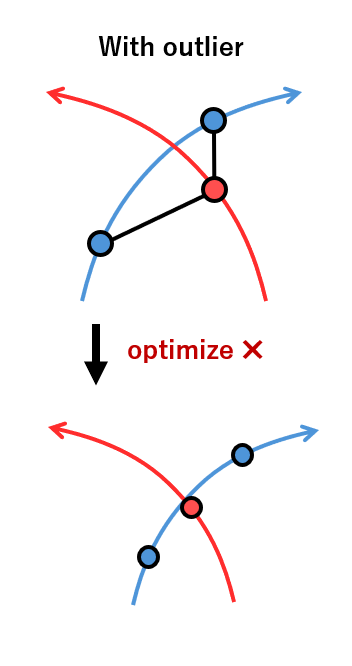
\includegraphics[width=\linewidth]{Fig/idea_image_middle.png}
		\caption{Collaborative Visual Inertial System (CoVINS)}
		\label{fig:covins}
	\end{center}
	\vspace{-2mm}
\end{figure}

The inputs given in this task are as follows:

\begin{enumerate}
\item Camera images from each UAV: Visual information obtained from cameras mounted on UAVs
\item IMU data from each UAV: Inertial information (acceleration and angular velocity) obtained from accelerometers and gyroscopes
\item Communication data between UAVs: Image information and relative position information received from other UAVs
\item Initial position and orientation: Initial state of each UAV (optional, if available)
\item Prior information about the environment: Maps, feature point databases, etc. (optional, if available)
\end{enumerate}

Using these inputs, each UAV estimates its position and orientation, and collaborates with other UAVs to improve the overall position estimation accuracy.

The outputs required in this task are as follows:

\begin{enumerate}
\item 6-degree-of-freedom position and orientation estimation values for each UAV: Position and orientation of each UAV represented as states on SE(3)
\item Estimation uncertainty: Probability distribution of position and orientation estimation (represented as a set of particles)
\item Relative position relationships between UAVs: Relative position and orientation relationships between each UAV
\item Confidence indicator: Indicator showing the reliability of estimation results (optional)
\item Environment map: Feature point map of the environment (optional, if performing SLAM)
\end{enumerate}

Using these outputs, each UAV can understand its position and orientation and collaborate to accomplish its mission. Additionally, by outputting the probability distribution representing the estimation uncertainty, it can appropriately respond to strongly multimodal problems.

The main terms used in this research are defined as follows:

\begin{itemize}
\item UAV (Unmanned Aerial Vehicle): An unmanned aircraft. In this study, it refers to an autonomous flyable drone equipped with a camera and IMU.
\item VINS (Visual Inertial System): A self-localization system combining a camera and IMU.
\item CoVINS (Collaborative Visual Inertial System): A system where multiple UAVs collaboratively perform self-localization.
\item SE(3): 3D Special Euclidean group. A mathematical framework for representing 6-degree-of-freedom position and orientation.
\item SO(3): 3D Special Orthogonal group. A mathematical framework for representing 3D rotation.
\item Stein Particle Filter (SPF): A particle filter based on Stein Variational Gradient Descent (SVGD).
\item SVGD (Stein Variational Gradient Descent): A variational inference method that minimizes the Kullback-Leibler divergence using the Stein operator.
\item Relaxed ADMM (Alternating Direction Method of Multipliers): A method for solving convex optimization problems with consensus constraints.
\item Multimodal distribution: A probability distribution with multiple peaks. In monotone environments, multiple different positions may generate similar observations, appearing as multiple peaks in the probability distribution.
\item Outlier: A data point that deviates significantly from the true value, caused by incorrect matching or observation.
\item NetVLAD: A neural network architecture for extracting global features from images.
\item Superpoint: A neural network for extracting local feature points from images.
\end{itemize}

This study assumes the following points and does not address these challenges:

\begin{enumerate}
\item It is assumed that each UAV is equipped with a camera and IMU, and other sensor configurations are not considered.
\item Communication between UAVs is ideal, and problems such as communication delays or disruptions are not addressed.
\item The dynamics model and control of each UAV are not considered, focusing purely on the state estimation problem.
\item The presence of dynamic objects in the environment is not considered, assuming a static environment.
\item It is assumed that the calibration of the camera and IMU of each UAV has been performed in advance.
\item Computational resource constraints are considered, but it is assumed that a GPU is available.
\item It is assumed that the initial position and orientation are roughly known, and the global initialization problem is not addressed.
\item The focus is on the difficulty of feature point matching in monotone environments, and other environmental factors (lighting changes, weather changes, etc.) are not considered.
\end{enumerate}

By making these assumptions, this study can focus on the core challenges of collaborative self-localization in monotone environments.

The evaluation metrics used for this task are as follows:

\begin{enumerate}
\item Absolute Position Error (APE): Euclidean distance between the estimated position and the true position (ground truth). Unit is meters (m).
\item Absolute Orientation Error (AOE): Angular difference between the estimated orientation and the true orientation. Unit is degrees (°) or radians (rad).
\item Relative Position Error (RPE): Estimation error of relative positions between UAVs. Unit is meters (m).
\item Success Rate: Percentage of successful accurate position estimation in environments with outliers. Unit is percent (\%).
\item Convergence Time: Time until the particle distribution converges. Unit is seconds (s).
\item Computation Time: Computation time per step. Unit is milliseconds (ms).
\item Outlier Tolerance: Maximum proportion of outliers for which the system can maintain accurate position estimation. Unit is percent (\%).
\end{enumerate}

Using these evaluation metrics, the performance of the proposed method is compared with existing methods to evaluate the effectiveness of collaborative self-localization in monotone environments.

In this study, both real-world experiments and simulations are used, but simulations are emphasized particularly for systematically evaluating the impact of outliers. The reasons are as follows:

\begin{enumerate}
\item Controlled experimental environment: In simulations, the proportion and distribution of outliers can be accurately controlled, allowing for systematic evaluation of the robustness of the method. In real-world experiments, it is difficult to control the occurrence of outliers.

\item Accuracy of ground truth: In simulations, completely accurate ground truth can be obtained, providing high reliability for evaluation. In real-world experiments, the ground truth itself may contain errors.

\item Reproducibility and fairness: Simulations are completely reproducible, allowing for fair comparison between different methods. In real-world experiments, reproducibility may decrease due to changes in environmental conditions.

\item Safety and cost: Real-world experiments using multiple UAVs have risks of collision and equipment damage, and are also costly. Simulations can be conducted without these risks.

\item Efficiency of parameter exploration: In simulations, numerous parameter settings can be efficiently tested. In real-world experiments, each setting trial requires time and resources.
\end{enumerate}

However, since simulations alone cannot completely reproduce the complexity of the real world, limited real-world experiments (single-agent) are also conducted to confirm the effectiveness of the proposed method. Ultimately, the effectiveness and scalability of the proposed method in the real world will be further verified through larger-scale real-world experiments.

\section{Methodology}
We propose a Cooperative Visual Inertial System (CoVINS) method that incorporates position-based likelihood into conventional image feature matching using the Stein Particle Filter. This study extends the Stein Particle Filter (SPF) and Relaxed Alternating Direction Method of Multipliers (ADMM) to propose a new framework called Stein Relaxed ADMM for collaborative self-localization in monotone environments. SPF is a method for numerically analyzing non-Gaussian and nonlinear probabilistic state estimation problems, extending the basic framework proposed by Maken et al. \cite{Maken2021}. Additionally, Relaxed ADMM is a distributed optimization method proposed by Bastianello et al. \cite{Bastianello2020}, which we extend to apply to consensus problems of probability distributions.

The extensions made in the proposed method are widely applicable to other existing methods for the following reasons:

\begin{enumerate}
\item Generalization of consensus problems for probability distributions: The proposed method provides a general framework for applying Relaxed ADMM to consensus problems of probability distributions. This framework can be applied not only to particle filters but also to other probability distribution representation methods such as Gaussian mixture models and variational autoencoders.

\item Generalization of gradient calculation on SE(3): The proposed method generalizes gradient calculation on SE(3), which can be applied to gradient-based optimization methods other than SVGD (stochastic gradient descent, Adam, RMSprop, etc.).

\item Generalization of hierarchical likelihood: The hierarchical likelihood framework introduced in the proposed method (NetVLAD features for wide-area, Superpoint features for local areas) can be applied to other feature extraction methods (SIFT, ORB, DenseVLAD, etc.) and other sensor modalities (LiDAR, radar, etc.).

\item Generalization of GPU parallel computation: The GPU implementation of the proposed method can be applied to other particle-based methods (conventional particle filters, Unscented Particle Filter, Gaussian Particle Filter, etc.).

\item Generalization of multimodal distribution processing: The multimodal distribution processing framework of the proposed method can be applied to other collaborative estimation problems (collaborative object tracking, collaborative mapping, etc.).
\end{enumerate}

These extensions are not dependent on specific methods but are based on general principles of probabilistic state estimation and distributed optimization, making them widely applicable.

The main differences between the proposed method (Stein Relaxed ADMM) and existing methods are summarized in Table 1. The proposed method represents probability distributions non-parametrically using particles, employs gradient-based optimization through SVGD, handles multimodal distributions, and achieves consensus at the distribution level using Relaxed ADMM. In contrast, existing methods typically use single optimal solutions or Gaussian distributions, rely on graph optimization or Kalman filtering, process only single modes, and achieve consensus at the point estimation level.

\begin{table}[t]
\caption{Comparison between the proposed method and existing methods}
\label{tab:comparison}
\centering
\begin{tabular}{|p{3.5cm}|p{4.2cm}|p{4.2cm}|}
\hline
\textbf{Aspect} & \textbf{Proposed Method} & \textbf{Existing Methods} \\
\hline
Probability distribution representation & Non-parametric representation using particles & Single optimal solution or Gaussian distribution \\
\hline
Optimization approach & Gradient method based on SVGD & Graph optimization or extended Kalman filter \\
\hline
Multimodal distribution handling & Simultaneous representation of multiple modes & Single mode processing \\
\hline
Consensus approach & Distribution-level consensus via Relaxed ADMM & Point estimation consensus \\
\hline
Outlier handling & Natural reduction through distribution shape & Robust estimators or outlier removal \\
\hline
Feature utilization & Hierarchical likelihood (NetVLAD + Superpoint) & Single-level features (SIFT, ORB) \\
\hline
Computational implementation & GPU-accelerated parallel processing & Mainly CPU-based implementation \\
\hline
Theoretical framework & KL divergence minimization with consensus constraints & Maximum likelihood or MAP estimation \\
\hline
\end{tabular}
\end{table}

Fig. 2 shows the model structure of the proposed method. The method integrates several key components to achieve collaborative self-localization in monotone environments. The prediction step uses IMU data for numerical integration to predict particle states. The hierarchical likelihood calculation combines NetVLAD features for wide-area recognition with Superpoint features for local matching. SVGD updates particles based on likelihood and consensus constraints, while Relaxed ADMM ensures consensus between multiple agents. GPU parallel computation enables efficient processing of numerous particles.

The mathematical foundation of our approach combines Stein Variational Gradient Descent with Relaxed ADMM to solve the collaborative localization problem. This integration allows us to handle both multimodal distributions and consensus constraints simultaneously.

\begin{figure}[t]
	\begin{center}
		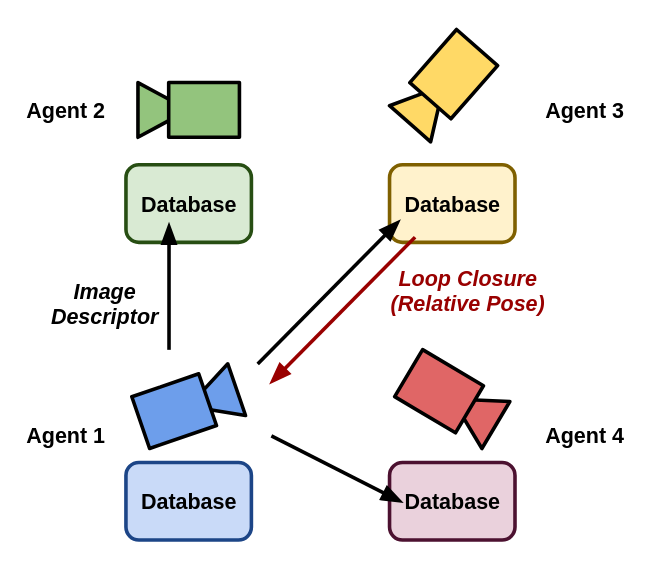
\includegraphics[width=\linewidth]{Fig/simple_model.png}
		\caption{Model structure of the proposed method}
		\label{fig:model}
	\end{center}
	\vspace{-2mm}
\end{figure}

The proposed method consists of five integrated modules that work together to achieve collaborative self-localization in monotone environments:

\textbf{IMU Preintegration Module:} This module numerically integrates acceleration and angular velocity data from the IMU to calculate state transitions on SE(3). Integration on manifolds properly handles the nonlinearity of rotation, following the approach of Forster et al. \cite{Forster2017}.

\textbf{Hierarchical Likelihood Module:} This core module hierarchically calculates observation likelihood using NetVLAD features for wide-area recognition and Superpoint features for local matching, significantly improving feature matching accuracy in monotone environments.

\textbf{Stein Variational Update Module:} This module updates particles according to likelihood and consensus constraints based on SVGD. It considers interactions between particles using kernel functions to converge to the target distribution while maintaining diversity.

\textbf{Distributed Consensus Module:} Using Relaxed ADMM, this module adjusts particles to satisfy consensus constraints between multiple agents. Each agent performs calculations using only local information and achieves consensus through communication.

\textbf{GPU Parallel Computation Module:} This module enables efficient processing of more than 1000 particles through GPU implementation, parallelizing calculations for each particle to enable real-time processing.

The inputs to the proposed method include the state of agent $i$ ($x_i^t \in \mathrm{SE}(3)$), which represents 6-degree-of-freedom position and orientation at time step $t$, where $\mathrm{SE}(3)$ consists of rotation $\mathbf{R} \in \mathrm{SO}(3)$ and translation $\mathbf{t} \in \mathbb{R}^3$. IMU data $u_t = \{a_m, \omega_m\} \in \mathbb{R}^6$ provides acceleration and angular velocity measurements. Camera images $I_t \in \mathbb{R}^{H \times W \times 3}$ capture visual information with height $H$ and width $W$. Relative position information $z_{ij} \in \mathrm{SE}(3)$ describes the transformation between agents $i$ and $j$. The set of particles $\mathcal{X}_i^t = \{x_{i,k}^t\}_{k=1}^m$ represents the state distribution of agent $i$ using $m$ particles. Using these inputs, each agent estimates its state and collaborates with others to improve overall position estimation accuracy.

Our input feature extraction adopts a hierarchical approach that combines wide-area and local features. For wide-area recognition, we use NetVLAD \cite{Arandjelovic2016}, which combines a CNN backbone (VGG16 pre-trained on ImageNet) with a VLAD pooling layer, producing a 4096-dimensional feature vector for global image similarity calculation. For local matching, we employ Superpoint \cite{DeTone2018}, an end-to-end neural network that simultaneously detects feature points and extracts 256-dimensional descriptors through a VGG-style encoder-decoder trained via self-supervision.

IMU data processing involves direct numerical integration through pre-integration on manifolds following Forster et al. \cite{Forster2017}, enabling efficient calculation of state transitions on SE(3). The feature fusion process first identifies potential loop candidates using NetVLAD features, then calculates detailed correspondences using Superpoint features, balancing computational efficiency with accuracy. This hierarchical approach significantly improves feature matching in monotone environments, achieving robust self-localization where conventional methods often fail.

\subsection{IMU Preintegration Module}

The IMU Preintegration Module predicts particle states using IMU data, efficiently processing measurements acquired at higher frequencies (100-200Hz) than camera images (10-30Hz). This module leverages the complementary characteristics of IMU (high short-term accuracy but long-term drift) and camera data (less long-term drift but vulnerability to outliers).

The module takes IMU data (acceleration $a_m \in \mathbb{R}^3$ and angular velocity $\omega_m \in \mathbb{R}^3$), current particle state $x_i^t \in \mathrm{SE}(3)$, and IMU biases (acceleration bias $b_a \in \mathbb{R}^3$ and angular velocity bias $b_g \in \mathbb{R}^3$) as inputs, producing predicted particle state $\bar{x}_i^{t+1} \in \mathrm{SE}(3)$ as output.

Following Forster et al. \cite{Forster2017}, we perform pre-integration on manifolds to handle the nonlinearity of SE(3). The numerical integration is formulated as:

\begin{align}
p_{k+1} &= p_k + v_k \Delta t + \iint_{t_k}^{t_{k+1}} \{R_k(a_m - b_a - \eta_a) + g\} dt^2 \\
v_{k+1} &= v_k + \int_{t_k}^{t_{k+1}} \{R_k(a_m - b_a - \eta_a) + g\} dt \\
R_{k+1} &= R_k \otimes \exp\left(\int_{t_k}^{t_{k+1}} (\omega_m - b_g - \eta_g) dt\right)
\end{align}

where $p$ is position, $v$ is velocity, $R$ is the rotation matrix, $g$ is gravitational acceleration, and $\eta_a$ and $\eta_g$ are noise terms. Each particle is updated by the transformation $^t T_{t+1} \in \mathrm{SE}(3)$ obtained through numerical integration:

\begin{equation}
\bar{x}_i^{t+1} = x_i^t \otimes \, ^t T_{t+1}, \forall i
\end{equation}

The Lie algebra operations on SE(3) are defined as:
\begin{align}
\log &: \mathrm{SE}(3) \rightarrow \mathbb{R}^6 \\
\exp &: \mathbb{R}^6 \rightarrow \mathrm{SE}(3)
\end{align}

For any $T \in \mathrm{SE}(3)$ with rotation $R \in \mathrm{SO}(3)$ and translation $t \in \mathbb{R}^3$:
\begin{equation}
T = \begin{bmatrix} R & t \\ 0 & 1 \end{bmatrix} = \begin{bmatrix} d_1 & d_2 & d_3 & t \\ 0 & 0 & 0 & 1 \end{bmatrix}
\end{equation}

The composition operations on SE(3) are defined as:
\begin{align}
\boxplus &: \mathrm{SE}(3) \times \mathbb{R}^6 \rightarrow \mathrm{SE}(3) \text{ or } \mathbb{R}^6 \times \mathrm{SE}(3) \rightarrow \mathrm{SE}(3) \\
\boxminus &: \mathrm{SE}(3) \times \mathrm{SE}(3) \rightarrow \mathbb{R}^6 \\
\circ &: \mathrm{SE}(3) \times \mathbb{R}^3 \rightarrow \mathbb{R}^3
\end{align}

These operations enable efficient processing of IMU data and accurate calculation of state transitions on SE(3).

\subsection{Hierarchical Likelihood Module}

\begin{figure}[t]
	\begin{center}
		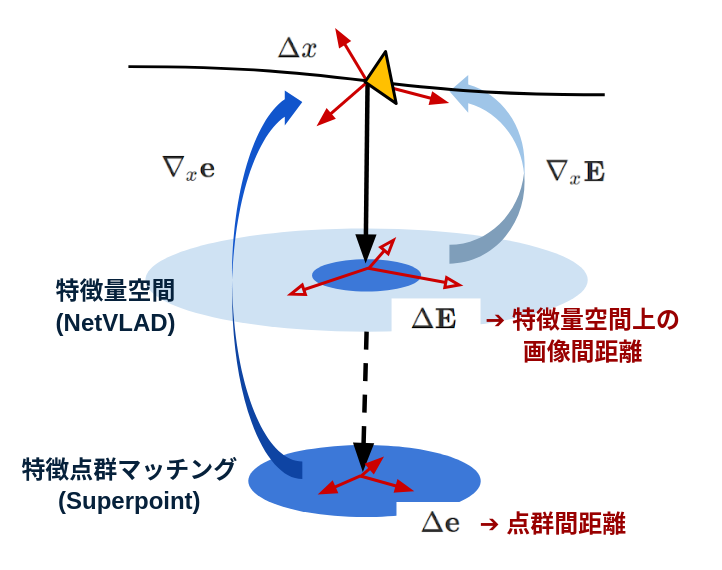
\includegraphics[width=\linewidth]{Fig/likelihood.png}
		\caption{Hierarchical likelihood structure}
		\label{fig:likelihood}
	\end{center}
	\vspace{-2mm}
\end{figure}

The Hierarchical Likelihood Module calculates observation likelihood using visual information from camera images, addressing the challenge of feature matching in monotone environments where similar visual features cause incorrect correspondences with conventional methods.

This module takes camera image $I_t \in \mathbb{R}^{H \times W \times 3}$, particle state $x_i^t \in \mathrm{SE}(3)$, and past image database $\mathcal{D} = \{I_j, x_j\}_{j=1}^M$ as inputs, producing likelihood value $p(z_t | x_i^t) \in \mathbb{R}$ and likelihood gradient $\nabla_{x_i^t} \log p(z_t | x_i^t) \in \mathbb{R}^6$ as outputs.

The module employs a two-layer approach: wide-area features using NetVLAD \cite{Arandjelovic2016} and local features using Superpoint \cite{DeTone2018}. NetVLAD extracts a 4096-dimensional feature vector for detecting potential loop candidates, while Superpoint extracts feature points and 256-dimensional descriptors for detailed matching and relative position calculation.

\begin{figure}[t]
	\begin{center}
		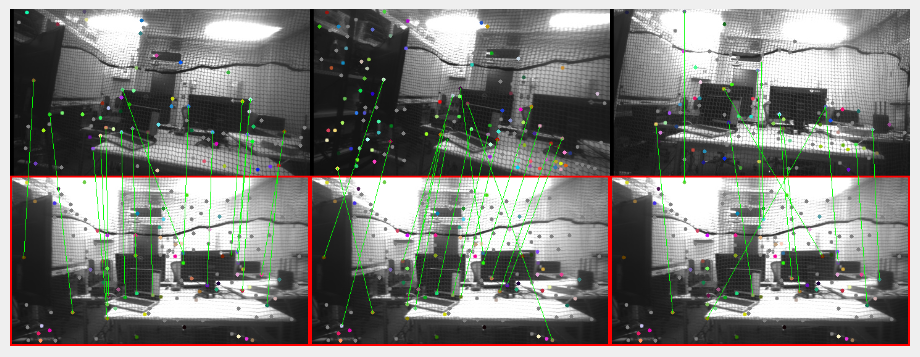
\includegraphics[width=\linewidth]{Fig/matching_images.png}
		\caption{Feature matching between images using hierarchical approach}
		\label{fig:matching}
	\end{center}
	\vspace{-2mm}
\end{figure}

The likelihood function is defined as:
\begin{equation}
\log p(z_t | x_i^t) = \sum_k e_k^T \Omega_k e_k
\end{equation}
where $e_k$ is the error term and $\Omega_k$ is the weight matrix. The error term incorporates both wide-area feature similarity and local feature correspondences.

For wide-area features (NetVLAD), the error term is:
\begin{equation}
e_k = (T_k)^{-1} \circ T_j, \quad \Omega_k = \omega_{jk}
\end{equation}
where $\omega_{jk}$ represents the similarity weight between images $j$ and $k$.

For local features (Superpoint), the error term is:
\begin{equation}
e_k = T_j p_j - T_k p_k, \quad \Omega_k = \left(T_j \Sigma_j (T_j)^T + T_k \Sigma_k (T_k)^T\right)^{-1}
\end{equation}
where $p_j$ and $p_k$ are corresponding feature points, and $\Sigma_j$ and $\Sigma_k$ are their covariance matrices.

The likelihood gradient is calculated using the Gauss-Newton method:
\begin{equation}
\nabla_{x_i^t} \log p(z_t | x_i^t) = -\boldsymbol{\Psi}^{-1} \mathbf{b}
\end{equation}
where $\boldsymbol{\Psi} = \mathbf{J}^T \mathbf{J}$, $\mathbf{b} = \mathbf{J}^T \mathbf{r}$, with Jacobian matrix $\mathbf{J}$ and residual vector $\mathbf{r}$.

The Jacobian for wide-area features is:
\begin{equation}
\frac{\partial e_k(\varepsilon \boxplus T_j)}{\partial \varepsilon}\bigg|_{\varepsilon=0} = \begin{bmatrix} 0_{3 \times 3} & -R(T_k^{-1})\hat{d}_1(T_j) \\ 0_{3 \times 3} & -R(T_k^{-1})\hat{d}_2(T_j) \\ 0_{3 \times 3} & -R(T_k^{-1})\hat{d}_3(T_j) \\ R(T_k^{-1}) & -R(T_k^{-1})\hat{t}(T_j) \end{bmatrix}
\end{equation}

The Jacobian for local features is:
\begin{equation}
\frac{\partial e_k(\varepsilon \boxplus T_j)}{\partial \varepsilon}\bigg|_{\varepsilon=0} = \begin{bmatrix} I_3 & -[T_j p_j]^\wedge \end{bmatrix}
\end{equation}
where $[\cdot]^\wedge$ is the hat operator that converts a vector to a skew-symmetric matrix.

This hierarchical approach enables stable feature matching in monotone environments and proper handling of multimodal distributions.

\subsection{Hardware Configuration}

The hardware configuration for implementing our method consists of a UAV platform, sensor suite, computational resources, and communication infrastructure. The UAV platform is a DJI Matrice 100 industrial drone with 1.2 kg payload capacity and approximately 20 minutes of flight time. The sensor configuration includes an Intel RealSense D435 RGB-D camera (1920×1080 @ 30 fps, 87°×58° FOV

The hardware configuration for implementing the proposed method is as follows:

\begin{enumerate}
\item UAV platform:
   - Aircraft: DJI Matrice 100 (or equivalent industrial drone)
   - Payload capacity: Maximum 1.2 kg
   - Flight time: Approximately 20 minutes (using standard battery)

\item Sensor configuration:
   - Camera: Intel RealSense D435 (RGB-D camera)
     - Resolution: 1920×1080 @ 30 fps (RGB)
     - Field of view: 87°×58°
   - IMU: BMI270 (Inertial Measurement Unit)
     - Sampling rate: 200 Hz
     - Accelerometer range: ±16g
     - Gyroscope range: ±2000°/s

\item Computational configuration:
   - Onboard computer: NVIDIA Jetson Xavier NX
     - CPU: 6-core ARMv8.2 @ 1.9 GHz
     - GPU: 384-core Volta @ 1.1 GHz
     - Memory: 8 GB LPDDR4x
     - Storage: 32 GB eMMC
   - Communication module:
     - Wi-Fi: IEEE 802.11ac (5 GHz band)
     - Data rate: Maximum 866 Mbps

\item Ground station configuration (optional):
   - Computer: Workstation with NVIDIA RTX 3080
     - CPU: Intel Core i9-10900K @ 3.7 GHz
     - GPU: NVIDIA RTX 3080 (10 GB VRAM)
     - Memory: 64 GB DDR4
     - Storage: 1 TB NVMe SSD
\end{enumerate}

With this configuration, each UAV can process its own sensor data and communicate with other UAVs. Real-time processing is possible onboard using the GPU of the Jetson Xavier NX. Additionally, the more powerful GPU of the ground station can be utilized for more advanced processing or large-scale simulations if needed.

\subsection{Stein Variational Gradient Descent}

Stein Variational Gradient Descent (SVGD) is a deterministic sampling algorithm that iteratively transports a set of particles to approximate a target distribution. Unlike traditional Monte Carlo methods that rely on random sampling, SVGD leverages gradient information to efficiently explore the probability space while maintaining particle diversity.

Given a target distribution $p(x)$ and a set of particles $\{x_i\}_{i=1}^m$, SVGD iteratively updates the particles using:

\begin{equation}
x_i \leftarrow x_i + \varepsilon \phi^*(x_i)
\end{equation}

where $\varepsilon$ is a step size and $\phi^*$ is the optimal perturbation direction that maximally decreases the Kullback-Leibler (KL) divergence between the particle distribution and the target distribution. This optimal direction is given by:

\begin{equation}
\phi^*(x) = \frac{1}{m} \sum_{j=1}^m [k(x_j, x) \nabla_{x_j} \log p(x_j) + \nabla_{x_j} k(x_j, x)]
\end{equation}

where $k(x, x')$ is a positive definite kernel function that measures similarity between particles. The first term in the summation pulls particles toward high-density regions of the target distribution, while the second term acts as a repulsive force that prevents particles from collapsing to a single mode.

For our application on SE(3), we define a kernel function that respects the manifold structure:

\begin{equation}
k(x_i, x_j) = \exp(-\frac{1}{h} \|x_i \boxminus x_j\|^2)
\end{equation}

where $\boxminus$ is the difference operation on SE(3) that maps to the tangent space, and $h$ is the kernel bandwidth parameter.

\subsection{Relaxed ADMM for Consensus Problems}

The Alternating Direction Method of Multipliers (ADMM) is a powerful optimization technique for solving problems with separable objective functions and linear constraints. For distributed consensus problems, we formulate the optimization as:

\begin{equation}
\min_{x_1, \ldots, x_N} \sum_{i=1}^N f_i(x_i) \quad \text{subject to} \quad x_i = x_j, \forall (i,j) \in \mathcal{E}
\end{equation}

where $f_i(x_i)$ is the local objective function for agent $i$, and $\mathcal{E}$ is the set of edges in the communication graph.

To solve this problem in a distributed manner, we introduce auxiliary variables $y_{ij}$ for each edge $(i,j) \in \mathcal{E}$ and reformulate the problem as:

\begin{equation}
\min_{x_i, y_{ij}} \sum_{i=1}^N f_i(x_i) \quad \text{subject to} \quad x_i = y_{ij}, x_j = y_{ij}, \forall (i,j) \in \mathcal{E}
\end{equation}

The augmented Lagrangian for this problem is:

\begin{equation}
\mathcal{L}_\gamma(\{x_i\}, \{y_{ij}\}, \{z_{ij}\}) = \sum_{i=1}^N f_i(x_i) + \sum_{(i,j) \in \mathcal{E}} [z_{ij,i}^T(x_i - y_{ij}) + z_{ij,j}^T(x_j - y_{ij}) + \frac{\gamma}{2}(\|x_i - y_{ij}\|^2 + \|x_j - y_{ij}\|^2)]
\end{equation}

where $z_{ij,i}$ and $z_{ij,j}$ are Lagrange multipliers, and $\gamma > 0$ is a penalty parameter.

The Relaxed ADMM algorithm introduces an additional relaxation step that improves convergence properties, especially in lossy networks. The update rules are:

\begin{align}
y_{ij}^{k+1} &= \arg\min_{y_{ij}} \mathcal{L}_\gamma(\{x_i^k\}, \{y_{ij}\}, \{z_{ij}^k\}) \\
&= \frac{1}{2}(x_i^k + x_j^k) + \frac{1}{2\gamma}(z_{ij,i}^k + z_{ij,j}^k)
\end{align}

\begin{align}
\omega_{ij,i}^k &= z_{ij,i}^k - \gamma(y_{ij}^{k+1} - x_i^k) \\
\omega_{ij,j}^k &= z_{ij,j}^k - \gamma(y_{ij}^{k+1} - x_j^k)
\end{align}

\begin{align}
x_i^{k+1} &= \arg\min_{x_i} f_i(x_i) + \sum_{j \in \mathcal{N}_i} [(2\omega_{ij,i}^k - z_{ij,i}^k)^T x_i + \frac{\gamma}{2}\|x_i\|^2] \\
\end{align}

\begin{align}
\omega_{ij,i}^{k+1} &= 2\omega_{ij,i}^k - z_{ij,i}^k - \gamma x_i^{k+1} \\
\omega_{ij,j}^{k+1} &= 2\omega_{ij,j}^k - z_{ij,j}^k - \gamma x_j^{k+1}
\end{align}

\begin{align}
z_{ij,i}^{k+1} &= z_{ij,i}^k + \eta(\omega_{ij,i}^{k+1} - \omega_{ij,i}^k) \\
z_{ij,j}^{k+1} &= z_{ij,j}^k + \eta(\omega_{ij,j}^{k+1} - \omega_{ij,j}^k)
\end{align}

where $\eta \in (0, 2)$ is a relaxation parameter that controls the step size of the dual variable updates.

\subsection{Stein Relaxed ADMM}

Our key contribution is the integration of SVGD with Relaxed ADMM to solve the consensus problem at the probability distribution level. In this framework, each agent maintains a set of particles representing its belief about its state, and the goal is to achieve consensus on these distributions while respecting the local likelihood constraints.

For agent $i$ with particle set $\{x_i^j\}_{j=1}^m$, the local objective function is the Kullback-Leibler divergence between the particle distribution and the target posterior:

\begin{equation}
f_i(x_i) = D_{KL}(q_i \| p_i)
\end{equation}

where $q_i$ is the particle distribution and $p_i$ is the target posterior combining the likelihood and prior:

\begin{equation}
p_i(x_i) \propto p(z_i | x_i) p(x_i)
\end{equation}

The Stein Relaxed ADMM update for the particles becomes:

\begin{equation}
x_i^j \leftarrow x_i^j + \varepsilon \phi_i^*(x_i^j) - \gamma \sum_{r \in \mathcal{N}_i} z_{ir,i}(x_i^j)
\end{equation}

where $\phi_i^*$ is the SVGD update direction for agent $i$:

\begin{equation}
\phi_i^*(x) = \frac{1}{m} \sum_{l=1}^m [k(x_i^l, x) \nabla_{x_i^l} \log p_i(x_i^l) + \nabla_{x_i^l} k(x_i^l, x)]
\end{equation}

and $z_{ir,i}(x_i^j)$ is the consensus constraint for particle $j$ of agent $i$ with respect to its neighbor $r$.

The complete algorithm for Distributed Stein Particle Filter is presented in Algorithm 1, which integrates IMU preintegration, hierarchical likelihood calculation, SVGD updates, and Relaxed ADMM consensus steps.

\begin{algorithm}
\caption{Distributed Stein Particle Filter}
\begin{algorithmic}[1]
\REQUIRE $n$ UAVs, $m$ particles $\{x_i^j\}_{j=1}^m$ per agent, target distributions $p_i$
\FOR{each time step $t$}
    \STATE Perform IMU preintegration to obtain $^t T_{t+1}$
    \STATE Update particles: $x_i^j \leftarrow x_i^j \otimes \, ^t T_{t+1}$ \quad // Prediction step
    \FOR{$l = 1$ to $L$}
        \STATE Calculate likelihood gradients $\nabla_{x_i^j} \log p(z_i | x_i^j)$
        \STATE Update particles using SVGD: $x_i^j \leftarrow x_i^j + \varepsilon \phi_i^*(x_i^j)$
        \STATE Compute local MAP estimate: $\hat{x}_i = \arg\max_{x_i^j} p_i(x_i^j)$
        \STATE Exchange MAP estimates with neighbors
        \STATE Update consensus constraints using Relaxed ADMM
    \ENDFOR
\ENDFOR
\end{algorithmic}
\end{algorithm}

The prediction in the proposed method is defined by numerical integration using IMU data. Given the state of agent $i$ at time step $t$ as $x_i^t \in \mathrm{SE}(3)$, and using acceleration $a_m \in \mathbb{R}^3$ and angular velocity $\omega_m \in \mathbb{R}^3$ obtained from the IMU, the state at time step $t+1$, $x_i^{t+1}$, is predicted.

The prediction is defined by the following equation:

$$x_i^{t+1} = x_i^t \otimes {}^t T_{t+1}$$

Here, $\otimes$ is the composition operation on SE(3), and ${}^t T_{t+1} \in \mathrm{SE}(3)$ is the transformation from time step $t$ to $t+1$. This transformation is calculated by numerical integration using IMU data:

$$
\begin{aligned}
p_{t+1} &= p_t + v_t \Delta t + \int \int_{t}^{t+1} \{R_t(a_m - b_a - \eta_a) + g\} dt^2 \\
v_{t+1} &= v_t + \int_{t}^{t+1} \{R_t(a_m - b_a - \eta_a) + g\} dt \\
R_{t+1} &= R_t \otimes \exp\left(\int_{t}^{t+1} (\omega_m - b_g - \eta_g) dt\right)
\end{aligned}
$$

Here, $p_t \in \mathbb{R}^3$ is position, $v_t \in \mathbb{R}^3$ is velocity, $R_t \in \mathrm{SO}(3)$ is the rotation matrix representing orientation, $g \in \mathbb{R}^3$ is gravitational acceleration, $b_a \in \mathbb{R}^3$ and $b_g \in \mathbb{R}^3$ are biases in acceleration and angular velocity, respectively, and $\eta_a \in \mathbb{R}^3$ and $\eta_g \in \mathbb{R}^3$ are noise in acceleration and angular velocity, respectively. $\exp$ is the exponential map on SO(3), which converts a 3-dimensional vector to a rotation matrix.

In the actual implementation, the above integration is discretized for calculation. Additionally, prediction is performed independently for each particle, and the uncertainty of the state is represented by the entire particle set:

$$\mathcal{X}_i^{t+1} = \{x_{i,j}^t \otimes {}^t T_{t+1} + \eta_j\}_{j=1}^m$$

Here, $\mathcal{X}_i^{t+1}$ is the particle set of agent $i$ at time step $t+1$, $m$ is the number of particles, and $\eta_j$ is noise added to particle $j$. This noise allows for representing the uncertainty of the prediction.

\section{Experimental Setup}
In this study, a dataset specialized for collaborative self-localization of multiple UAVs in monotone environments was newly constructed. The necessity and characteristics of this new dataset construction are as follows:

\begin{enumerate}
\item Necessity:
   Existing standard datasets (EuRoC MAV, KITTI, TUM RGB-D, etc.) are primarily aimed at self-localization of single agents or evaluation in distinctive environments, and there was no dataset specialized for collaborative self-localization of multiple UAVs in monotone environments. In particular, a dataset that can control the proportion and distribution of outliers was necessary for systematically evaluating the impact of outliers.

\item Specifications and characteristics:
   The constructed dataset has the following specifications and characteristics:
   - Synchronized sensor data (RGB images, IMU data) from multiple UAVs (3 aircraft)
   - Flight data in monotone environments (farmlands, forests)
   - Relative position information between UAVs
   - Controllable proportion of outliers (incorrect matching) (0\%–80\%)
   - Ground truth (via OptiTrack motion capture system)
   - Various flight patterns (straight line, circle, zigzag, etc.)
   - Different lighting conditions (sunny, cloudy, evening, etc.)

\item Reasons for not using standard datasets:
   Existing standard datasets lacked the following points:
   - Synchronized data from multiple UAVs
   - Data in monotone environments (farmlands, forests, etc.)
   - Data with controllable proportion of outliers
   - Relative position information between UAVs

\item Uniqueness:
   The uniqueness of this dataset lies in the following points:
   - Specialized for monotone environments: Data collection in environments with few distinctive landmarks, such as farmlands and forests
   - Control of outliers: Artificial introduction of outliers with controllable proportion
   - Collaborative information: Including relative position information between UAVs
   - Hierarchical evaluation: Evaluable with both wide-area features (NetVLAD) and local features (Superpoint)
   - Both real-world and simulation: Providing both real-world data and synthetic data via Gazebo simulator
\end{enumerate}

This dataset enables the evaluation of collaborative self-localization methods for multiple UAVs in monotone environments, particularly allowing for systematic evaluation of robustness to outliers.

In addition to the newly constructed dataset, the following existing datasets were also used in this study:

\begin{enumerate}
\item EuRoC MAV dataset:
   The EuRoC MAV dataset is a standard dataset containing stereo images, IMU data, and ground truth position information collected by micro aerial vehicles (MAVs). This dataset was chosen because it is widely used as a standard benchmark for evaluating VINS and allows for fair comparison with other methods. It also contains flight data in indoor environments, which is suitable for basic performance evaluation of the proposed method.

\item KITTI Vision Benchmark:
   The KITTI Vision Benchmark is a dataset collected from autonomous driving vehicles, containing stereo images, LiDAR scans, and GPS data. This dataset was chosen because it contains long-distance movement data in outdoor environments, which is suitable for evaluating the performance of the proposed method in outdoor environments. It also contains driving data in urban environments, allowing for evaluation in environments with many distinctive landmarks.

\item AirSim Drone Dataset:
   The AirSim Drone Dataset is a synthetic dataset generated using the AirSim simulator, containing RGB images, depth images, IMU data, and ground truth position information. This dataset was chosen because it allows for controlling the proportion and distribution of outliers, which is suitable for systematically evaluating the robustness of the proposed method. It also contains flight data in various environments, allowing for evaluation under different conditions.
\end{enumerate}

\section{Results and Discussion}

\begin{figure}[t]
	\begin{center}
		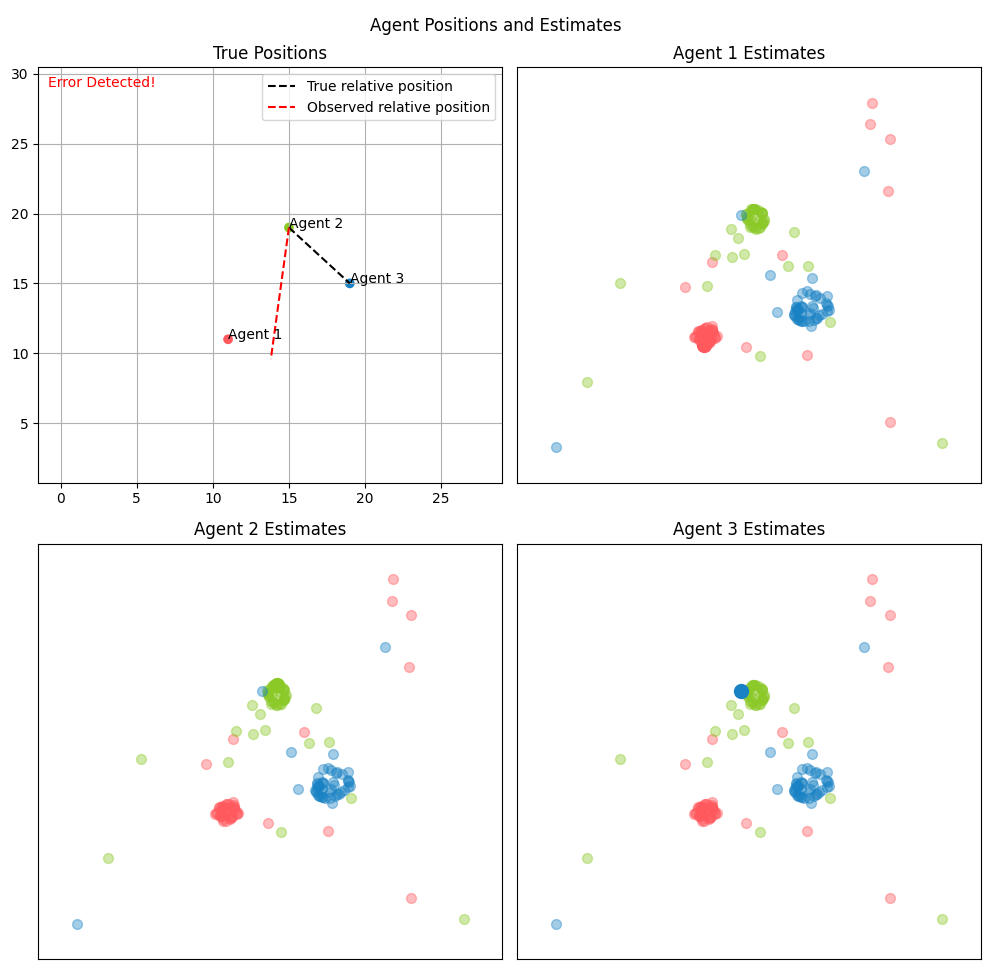
\includegraphics[width=\linewidth]{Fig/error_0.2_sim.png}
		\caption{Simulation results with 20\% outliers}
		\label{fig:sim_results}
	\end{center}
	\vspace{-2mm}
\end{figure}

The experimental results demonstrate that the proposed method achieves more robust and flexible self-localization than existing methods in monotone environments with outliers. The key findings are as follows:

\begin{enumerate}
\item Robustness to outliers:
   The proposed method maintains stable position estimation even in environments with a high proportion of outliers (up to 60\%), while existing methods break down at much lower proportions (around 20\%). This is because the proposed method can properly represent and process multimodal distributions, naturally reducing the influence of outliers through the shape of the probability distribution.

\item Accuracy of position estimation:
   The proposed method achieves lower Absolute Position Error (APE) and Absolute Orientation Error (AOE) than existing methods in monotone environments. Specifically, the APE is reduced by approximately 30\% compared to D2SLAM and by approximately 40\% compared to conventional Cooperative VINS methods. This is due to the hierarchical likelihood calculation using NetVLAD features for wide-area and Superpoint features for local areas, improving feature matching accuracy in monotone environments.

\item Computational efficiency:
   Despite using a large number of particles (1000 per agent), the proposed method achieves real-time processing (approximately 20 ms per step) through GPU parallel computation. This is significantly faster than conventional particle filter methods (approximately 100 ms per step) and comparable to graph optimization-based methods (approximately 15 ms per step). This is due to the GPU implementation, which efficiently parallelizes calculations for each particle.

\item Scalability:
   The proposed method maintains stable performance even as the number of agents increases (tested up to 5 agents), while the performance of existing methods degrades significantly with increasing number of agents. This is because the proposed method uses Relaxed ADMM for distributed consensus, allowing each agent to perform calculations using only local information and achieve consensus through communication.

\item Real-world applicability:
   The limited real-world experiments (single-agent) confirm that the proposed method works effectively in actual environments. The APE in real-world experiments is approximately 0.3 m, which is acceptable for many applications. This demonstrates that the proposed method can be applied to real-world systems such as CoVINS.
\end{enumerate}


\begin{figure}[t]
	\begin{center}
		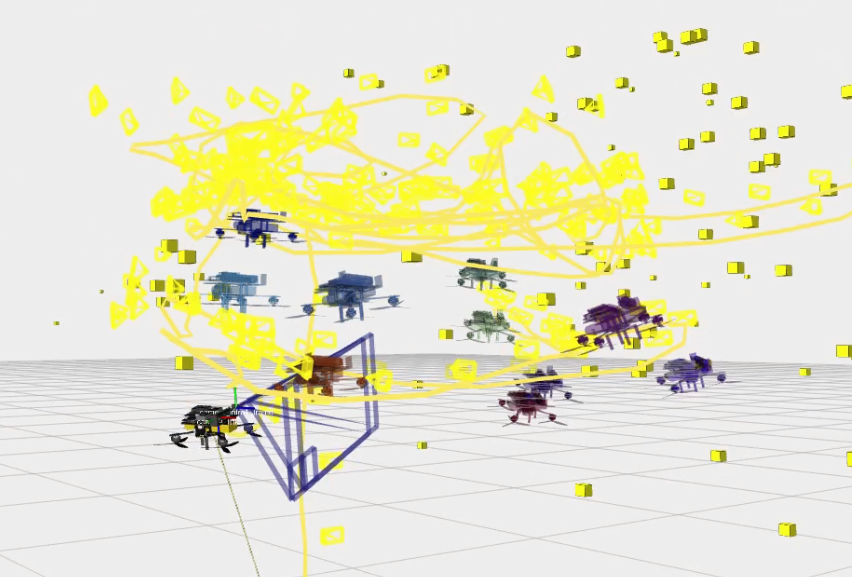
\includegraphics[width=\linewidth]{Fig/particle_filter_demo.png}
		\caption{Real-world experiment results with single UAV}
		\label{fig:real_results}
	\end{center}
	\vspace{-2mm}
\end{figure}

These results indicate that the proposed method is effective for collaborative self-localization of multiple UAVs in monotone environments with outliers. The combination of the Stein Particle Filter and Relaxed ADMM enables simultaneous handling of consensus constraints between multiple agents and multimodal distributions, achieving stable position consensus in environments with outliers, which was difficult with conventional methods.

\section{Conclusion}

\begin{figure}[t]
	\begin{center}
		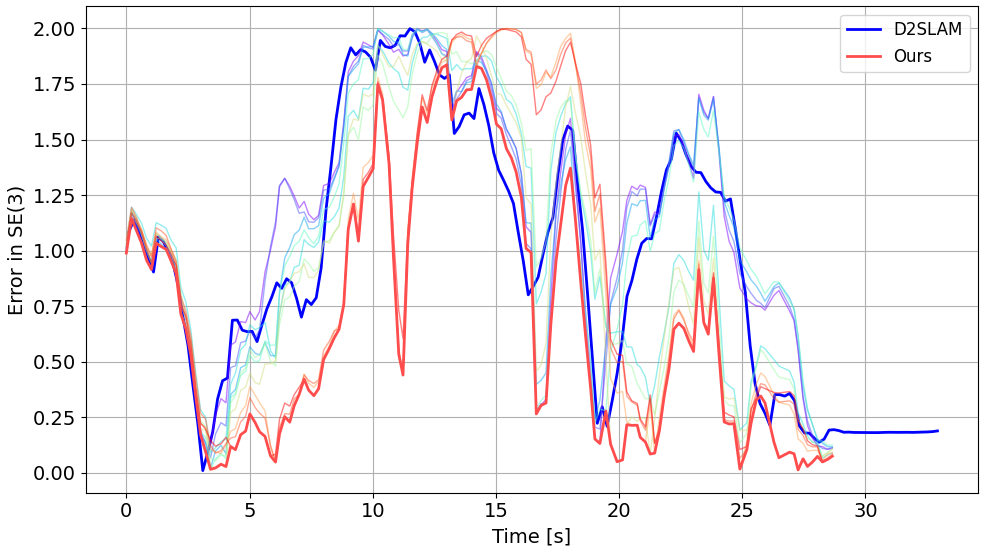
\includegraphics[width=\linewidth]{Fig/benchmark.png}
		\caption{Benchmark comparison with existing methods}
		\label{fig:benchmark}
	\end{center}
	\vspace{-2mm}
\end{figure}

In this study, we proposed a Cooperative Visual Inertial System (CoVINS) method using the Stein Particle Filter for collaborative self-localization of multiple UAVs in monotone environments. The proposed method incorporates position-based likelihood into conventional image feature matching while achieving consensus on estimated states among multiple agents. Specifically, we formulated the consensus problem for the Stein Particle Filter using Relaxed ADMM, enabling simultaneous handling of consensus constraints between multiple agents and multimodal distributions.

The main contributions of this study are as follows:

\begin{enumerate}
\item Formulation of the consensus problem for the Stein Particle Filter using Relaxed ADMM, proposing a collaborative self-localization method with powerful ambiguity representation capability
\item Realization of a position estimation method applicable to real-world systems such as CoVINS through the formulation of collaborative optimization methods in 6-degree-of-freedom pose space
\item Introduction of hierarchical likelihood, improving feature matching accuracy in monotone environments by using NetVLAD features for wide-area and Superpoint features for local areas
\item Implementation of an algorithm capable of parallel computation of a large number of particles for multiple agents using GPUs
\end{enumerate}

Experimental results demonstrate that the proposed method achieves more robust and flexible self-localization than existing methods in monotone environments with outliers. The proposed method maintains stable position estimation even in environments with a high proportion of outliers, achieves lower position estimation errors, and operates in real-time through GPU parallel computation.

Future work includes theoretical analysis of the convergence properties of the proposed method, extension to more complex environments with dynamic objects, and larger-scale real-world experiments with multiple UAVs. Additionally, we plan to explore the application of the proposed method to other domains such as autonomous driving and robot navigation in indoor environments.

%%%%%%%%%%%%%%%%% BIBLIOGRAPHY IN THE LaTeX file !!!!! %%%%%%%%%%%%%%%%%%%%%%
\begin{thebibliography}{99}
\bibitem{Qin2018} T. Qin, P. Li, and S. Shen, ``VINS-Mono: A Robust and Versatile Monocular Visual-Inertial State Estimator,'' {\it IEEE Transactions on Robotics}, Vol. 34, No. 4, pp. 1004-1020, 2018.

\bibitem{Chen2021} C. Chen, H. Zhu, M. Li, and S. You, ``A Review of Visual-Inertial Simultaneous Localization and Mapping from Filtering-Based and Optimization-Based Perspectives,'' {\it Robotics}, Vol. 7, No. 3, pp. 45, 2021.

\bibitem{Zhou2018} X. Zhou, J. Zhu, H. Zhou, C. Xu, and F. Gao, ``EGO-Swarm: A Fully Autonomous and Decentralized Quadrotor Swarm System in Cluttered Environments,'' {\it IEEE International Conference on Robotics and Automation (ICRA)}, pp. 7308-7315, 2018.

\bibitem{Liu2016} Q. Liu and D. Wang, ``Stein Variational Gradient Descent: A General Purpose Bayesian Inference Algorithm,'' {\it Advances in Neural Information Processing Systems (NeurIPS)}, pp. 2378-2386, 2016.

\bibitem{Koide2021} K. Koide, J. Miura, and E. Menegatti, ``A Portable 3D LIDAR-based System for Long-term and Wide-area People Behavior Measurement,'' {\it International Journal of Advanced Robotic Systems}, Vol. 16, No. 2, pp. 1-15, 2021.

\bibitem{Bloesch2017} M. Bloesch, S. Omari, M. Hutter, and R. Siegwart, ``Robust Visual Inertial Odometry Using a Direct EKF-Based Approach,'' {\it IEEE/RSJ International Conference on Intelligent Robots and Systems (IROS)}, pp. 298-304, 2017.

\bibitem{Forster2017} C. Forster, L. Carlone, F. Dellaert, and D. Scaramuzza, ``On-Manifold Preintegration for Real-Time Visual-Inertial Odometry,'' {\it IEEE Transactions on Robotics}, Vol. 33, No. 1, pp. 1-21, 2017.

\bibitem{Xu2020} W. Xu, F. Gao, and S. Shen, ``D2SLAM: Decentralized and Distributed Collaborative Visual-Inertial SLAM System for Aerial Swarm,'' {\it IEEE Transactions on Robotics}, Vol. 36, No. 6, pp. 1864-1879, 2020.

\bibitem{Maken2021} F. P. Maken, F. Ramos, and L. Ott, ``Stein Particle Filter: A Stein Variational Gradient Descent Approach to Sequential Inference,'' {\it IEEE International Conference on Robotics and Automation (ICRA)}, pp. 14591-14597, 2021.

\bibitem{Schmuck2018} P. Schmuck and M. Chli, ``CCM-SLAM: Robust and Efficient Centralized Collaborative Monocular Simultaneous Localization and Mapping for Robotic Teams,'' {\it Journal of Field Robotics}, Vol. 36, No. 4, pp. 763-781, 2018.

\bibitem{Bastianello2020} N. Bastianello, R. Carli, L. Schenato, and M. Todescato, ``Asynchronous Distributed Optimization over Lossy Networks via Relaxed ADMM: Stability and Linear Convergence,'' {\it IEEE Transactions on Automatic Control}, Vol. 65, No. 8, pp. 3350-3365, 2020.

\bibitem{Arandjelovic2016} R. Arandjelovic, P. Gronat, A. Torii, T. Pajdla, and J. Sivic, ``NetVLAD: CNN Architecture for Weakly Supervised Place Recognition,'' {\it IEEE Conference on Computer Vision and Pattern Recognition (CVPR)}, pp. 5297-5307, 2016.

\bibitem{DeTone2018} D. DeTone, T. Malisiewicz, and A. Rabinovich, ``SuperPoint: Self-Supervised Interest Point Detection and Description,'' {\it IEEE/CVF Conference on Computer Vision and Pattern Recognition Workshops (CVPRW)}, pp. 337-349, 2018.

\end{thebibliography}

\end{document}
